\subsection{Đánh giá định lượng giải thích XAI}\label{sec:r-xai}
Nhóm đánh giá liệu cạnh được chọn để giải thích ảnh đứng đầu có ảnh hưởng đến quyết định của QA-Graph hay không. Hai lượt đánh giá dùng checkpoint đã huấn luyện trên VG$\cap$COCO và PSG$\cap$COCO, mỗi bộ có ba seed. Ở mọi phép can thiệp, 100 ảnh ứng viên được giữ cố định và điểm của chúng được tính lại. Lượt khảo sát gồm 12 caption mỗi bộ, được chọn theo nhóm truy vấn và kết quả ở seed 0; lượt tập trung vào 18 truy vấn trực tiếp VG và 16 truy vấn trực tiếp PSG có ảnh chuẩn đã được xác nhận hỗ trợ truy vấn. Đây là các mẫu phân tích có chủ đích, không phải mẫu ngẫu nhiên của toàn bộ tập test.

Ký hiệu $s(q,i;G)$ là điểm xếp hạng~(\ref{eq:fuse}) khi QA-Graph~(\ref{eq:qa}) dùng đồ thị $G$; sau mỗi can thiệp, điểm QA-Graph và bước chuẩn hóa được tính lại trên đúng 100 ảnh ứng viên.

Gọi $E$ là các cạnh giải thích được xóa đồng thời, $E_{\mathrm{eligible}}$ là tập cạnh đủ điều kiện xem xét và $R_b$ là tập cạnh đối chứng thứ $b$, cùng số cạnh với $E$: ở lượt khảo sát là cạnh ngẫu nhiên cùng loại (20 tập), ở lượt truy vấn trực tiếp là các cạnh đối tượng khác của chính ảnh đó. Các độ đo trên một cặp truy vấn--ảnh được xác định như sau:
\begin{align}
d_E(q,i) &= s(q,i;G)-s(q,i;G\setminus E), \label{eq:xai-drop}\\
F(q,i) &= d_E(q,i)-\overline{d_R(q,i)}, \label{eq:xai-fidelity}\\
S(q,i) &= 1-\frac{|E|}{|E_{\mathrm{eligible}}|}, \label{eq:xai-sparsity}\\
V_{\mathrm{str}}(q,i) &= \frac{|E_{\mathrm{valid}}|}{|E|}. \label{eq:xai-validity}
\end{align}
Ở đây, $\overline{d_R(q,i)}$ là mức giảm điểm trung bình khi xóa các tập $R_b$; $E_{\mathrm{valid}}$ gồm những cạnh tồn tại trong đồ thị và đúng kiểu đỉnh, chiều cạnh. Lợi thế fidelity dương nghĩa là cạnh giải thích ảnh hưởng đến điểm xếp hạng mạnh hơn đối chứng. Sparsity và validity cấu trúc chỉ tính khi có giải thích; kiểm tra đường đi hợp lệ được báo riêng. Các mức giảm điểm thuộc thang của tổng hai thành phần đã chuẩn hóa, không phải phần trăm hay mức tăng MRR. Validity thị giác của từng cạnh cần bằng chứng từ ảnh ngoài phép kiểm tra cấu trúc này.

\textbf{Lượt khảo sát.} Mỗi bộ có 12 caption được đánh giá trên ba seed với ngân sách một, ba hoặc năm cạnh; đối chứng là 20 tập cạnh ngẫu nhiên. Ở ngân sách ba cạnh, xóa cạnh giải thích làm điểm ảnh đứng đầu giảm trung bình $0{,}902$ trên VG, so với $0{,}173$ của đối chứng; lợi thế là $0{,}729$ (CI95 $[0{,}561;0{,}931]$). Trên PSG, các giá trị tương ứng là $1{,}723$, $0{,}726$ và $0{,}996$ (CI95 $[0{,}878;1{,}104]$). Hình~\ref{fig:xai-baseline} cho thấy lợi thế dương ở cả ba ngân sách. Tuy nhiên, sau can thiệp ảnh chuẩn chỉ tăng hạng trong 7/36 trường hợp VG và 18/36 trường hợp PSG ở ngân sách ba cạnh: làm yếu ảnh đang đứng đầu không bảo đảm ảnh chuẩn được đưa lên cao hơn.

\begin{figure*}[t]
\centering
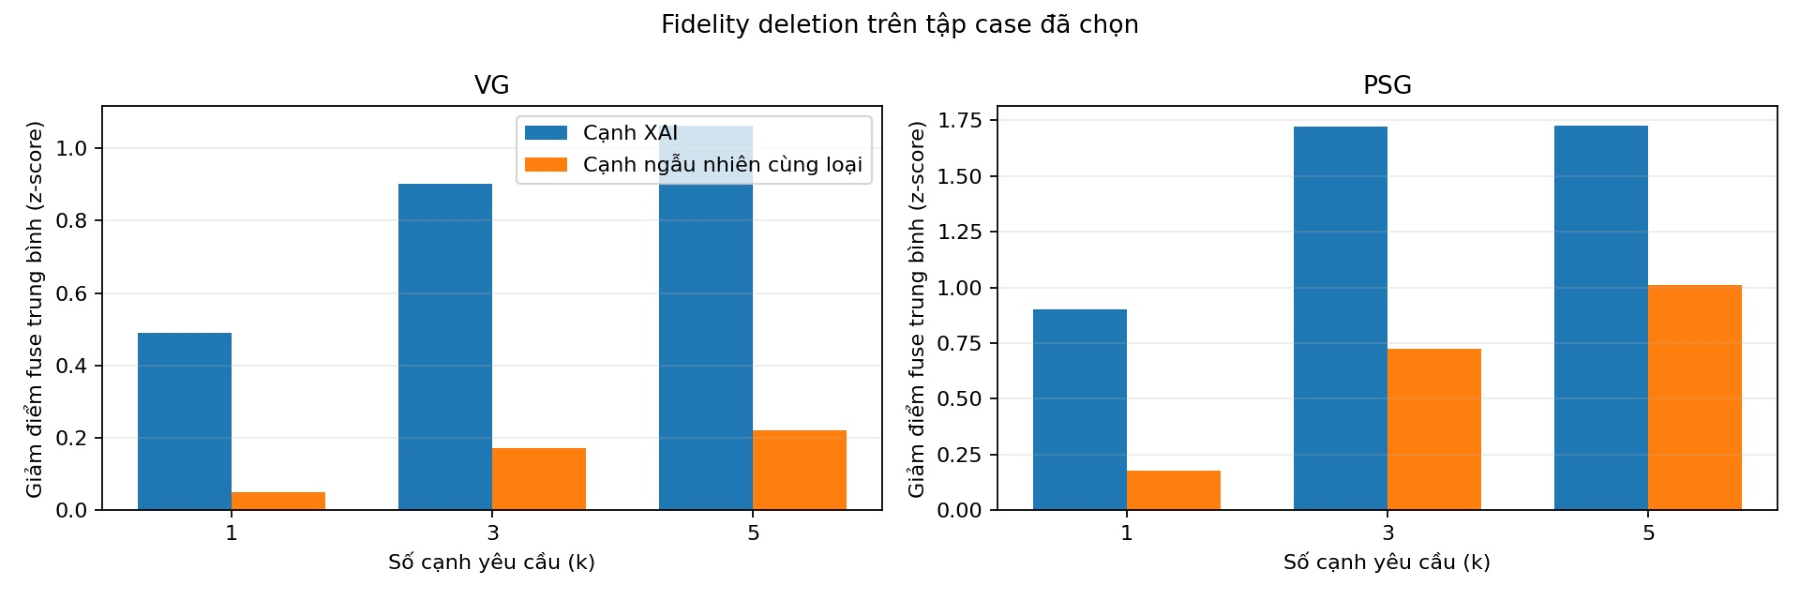
\includegraphics[width=\textwidth]{figs/xai_baseline_fidelity.pdf}
\caption{Mức giảm điểm xếp hạng của ảnh đứng đầu khi xóa cạnh giải thích và cạnh đối chứng trên mẫu 12 caption mỗi bộ dữ liệu, ba seed, 20 phép đối chứng cho mỗi trường hợp. So sánh hai cột trong cùng bộ dữ liệu; thang điểm của VG và PSG khác nhau.}\label{fig:xai-baseline}
\end{figure*}

\textbf{Lượt truy vấn trực tiếp.} Bộ giải thích chọn cạnh đối tượng nối nhãn phù hợp với truy vấn tới ảnh đứng đầu. Bảng~\ref{tab:xai-direct} cho thấy lợi thế fidelity dương ở mọi ngân sách có đối chứng. Tại ba cạnh, 51/54 trường hợp VG và 48/48 trường hợp PSG có giải thích; lợi thế trung bình lần lượt là $0{,}646$ và $1{,}094$. Ba trường hợp VG không có cạnh phù hợp đều thuộc cùng một truy vấn ở ba seed và vẫn nằm trong mẫu số độ bao phủ. Ba trường hợp PSG tại ngân sách ba cạnh thiếu tập đối chứng độc lập; chúng không được gán lợi thế bằng không. CI95 được bootstrap theo truy vấn, giữ các seed của cùng truy vấn trong một cụm. Lợi thế fidelity chỉ tính cho các trường hợp có đối chứng, còn sparsity chỉ tính khi có giải thích.

\begin{table*}[t]
\caption{Đánh giá trên 34 truy vấn trực tiếp đã duyệt, ba seed cho mỗi bộ dữ liệu. Lợi thế fidelity là mức giảm điểm của ảnh đứng đầu khi xóa cạnh giải thích trừ mức giảm khi xóa cạnh đối chứng cùng ảnh; CI95 lấy mẫu theo truy vấn. Sparsity tính trên các cạnh đối tượng đủ điều kiện của ảnh.}\label{tab:xai-direct}
\centering\small
\begin{tabular}{lccccc}
\toprule
Bộ dữ liệu & Số cạnh & Có giải thích & Có đối chứng & Lợi thế fidelity [CI95] & Sparsity (\%)\\\midrule
VG$\cap$COCO & 1 & 51/54 & 51/54 & $0{,}348$ $[0{,}264;0{,}436]$ & 93,5\\
VG$\cap$COCO & 2 & 51/54 & 51/54 & $0{,}538$ $[0{,}404;0{,}667]$ & 88,7\\
VG$\cap$COCO & 3 & 51/54 & 51/54 & $0{,}646$ $[0{,}481;0{,}818]$ & 85,7\\
PSG$\cap$COCO & 1 & 48/48 & 48/48 & $0{,}583$ $[0{,}500;0{,}660]$ & 82,4\\
PSG$\cap$COCO & 2 & 48/48 & 48/48 & $1{,}070$ $[0{,}818;1{,}342]$ & 68,9\\
PSG$\cap$COCO & 3 & 48/48 & 45/48 & $1{,}094$ $[0{,}831;1{,}388]$ & 66,4\\\bottomrule
\end{tabular}
\end{table*}

Hình~\ref{fig:xai-direct} đặt fidelity cạnh độ bao phủ và sparsity để tránh diễn giải mức giảm điểm mà bỏ qua các trường hợp không tìm được giải thích. Lợi thế so với cạnh ngẫu nhiên là thống kê có điều kiện: bộ giải thích đã chọn cạnh theo chính mức giảm điểm, nên đối chứng này không phải kiểm định độc lập về độ đúng ngữ nghĩa. Sparsity giảm khi ngân sách cạnh tăng, như dự kiến từ định nghĩa.

\begin{figure*}[t]
\centering
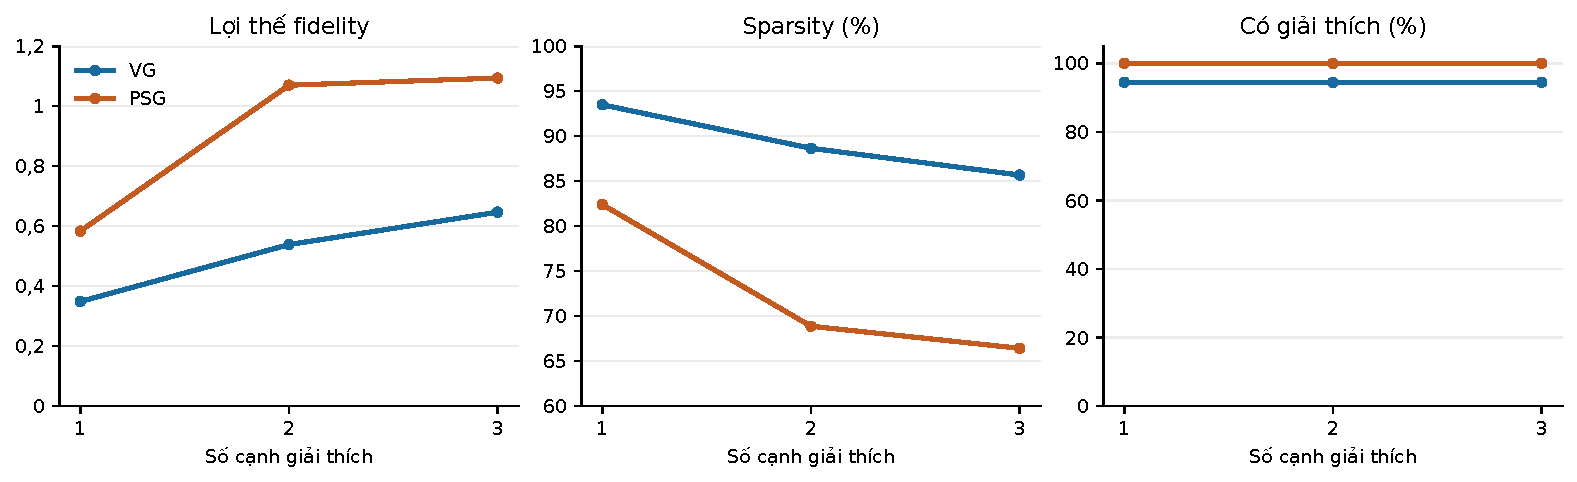
\includegraphics[width=\textwidth]{figs/xai_direct_metrics.pdf}
\caption{Lợi thế fidelity, sparsity và tỷ lệ trường hợp có giải thích ở lượt truy vấn trực tiếp. Fidelity chỉ tính nơi có đối chứng; tỷ lệ có giải thích tính trên mọi trường hợp đã đăng ký. Mỗi bộ dữ liệu có ba seed; thang điểm fidelity giữa hai bộ không dùng để so chất lượng mô hình.}\label{fig:xai-direct}
\end{figure*}

\textbf{Validity và phạm vi diễn giải.} Trong lượt khảo sát, validity cấu trúc của cạnh và đường đi đều đạt 216/216 lượt; đây là kiểm tra lược đồ, không phải xác nhận bằng thị giác. Tỷ lệ cạnh có trạng thái bằng chứng đã được kiểm chứng là 0 vì metadata còn ở trạng thái chưa xác định. Ở ngân sách ba cạnh, 102/108 cạnh VG và 104/108 cạnh PSG được chọn là cạnh nối nhãn với ảnh; chỉ có 6 và 4 đường đi dài hai cạnh tương ứng. Kết quả vì vậy chủ yếu cho thấy mô hình phụ thuộc vào tín hiệu đối tượng. Việc xem ảnh ở mục~\ref{sec:cases} đánh giá riêng mức phù hợp của ảnh đứng đầu đối với truy vấn, không thay thế kiểm tra từng cạnh hay quan hệ trong ảnh.
